% !TeX program = xelatex
\documentclass[statementpaper,12pt,extrafontsizes%,openright,openleft
,openany%,draft,showtrims,twoside
]{memoir}
\setstocksize{7.5in}{5.5in}
\settrimmedsize{\stockheight}{\stockwidth}{*}
%\setsecnumdepth{subsubsection}
\setcounter{tocdepth}{3}


%\setpagebl{16cm}{12cm}{*}
\settypeblocksize{28\baselineskip}{3.7in}{*}
%\setulmargins{50pt}{*}{*}
%\semiisopage[10]
%\setbinding{0.3in}
\setlrmargins{*}{*}{*}
%\setlrmarginsandblock{0.75in}{0.15in}{*}
\setulmargins{1in}{*}{*}
%\setmarginnotes{0pt}{0pt}{*}
%\setlength\marginparwidth {0pt}
%\setlength\marginparsep {0pt}
%\settrims{0pt}{0pt}
\setheaderspaces{*}{12pt}{*}
\setheadfoot{\onelineskip}{1.5\onelineskip}

%% set up the recto page layout
\checkandfixthelayout[lines]
\setlength{\evensidemargin}{\oddsidemargin}% after \checkandfix

%%%%%%%%%%%%        Define The Custom Chapter Style %%%%%%%%%%%%
%% gurusimple1 chapter style
\makechapterstyle{gurusimple1}{%
	\setlength{\beforechapskip}{3\onelineskip}%
	\renewcommand{\printchaptertitle}[1]{\centering\Large\bfseries{##1}}
	\renewcommand{\afterchaptertitle}{\vskip\onelineskip
		\hrule\vskip\onelineskip}
%	\renewcommand*{\chapterheadstart}{\vspace{5\beforechapskip}}%
%	\setlength{\afterchapskip}{2\onelineskip \@plus .2\onelineskip \@minus 0.2\onelineskip}%
%	\renewcommand*{\printchaptername}{}%
%	\renewcommand*{\chapternamenum}{}%
	\renewcommand*{\chapnumfont}{\normalfont\Large\bfseries}%
	\renewcommand*{\chaptitlefont}{\chapnumfont}%
	\renewcommand*{\chapnamefont}{\chapnumfont}%
%	\renewcommand*{\printchapternum}{%
%		\centering\chapnumfont \chapternamenum\thechapter\quad}%
%	\renewcommand{\afterchapternum}{}%
%	\renewcommand*{\printchapternonum}{\centering}
}

\makeheadstyles{gurusimple1}{%
	\chapterstyle{gurusimple1}
	\setsecheadstyle{\large\bfseries\centering}%
	\setsubsecheadstyle{\normalsize\bfseries\centering}%
	\setsubsubsecheadstyle{\normalsize\itshape\centering}%
%	\setparaheadstyle{\normalfont\normalsize\centering\itshape}%
%	\setsubparaindent{\parindent}%
%	\setsubparaheadstyle{\normalfont\normalsize\scshape\MakeTextLowercase}
}

%\chapterstyle{gurusimple1}
%\chapterstyle{crosshead}
\headstyles{gurusimple1}

%%%%%%%%%%%%     End of Custom Chapter Style %%%%%%%%%%%%

%\setafterSskip{\onelineskip}

\makepagestyle{mystyle}
%\setlength{\headwidth}{\dimexpr\textwidth+\marginparsep+\marginparwidth\relax}
%\makerunningwidth{mystyle}{\headwidth}
\makeevenhead{mystyle}{\itshape\thepage}{}{\itshape\rightmark}
\makeoddhead{mystyle}{\itshape\leftmark}{}{\itshape\thepage}
\makeevenfoot{mystyle}{}{}{}
\makeoddfoot{mystyle}{}{}{}
\makepsmarks{mystyle}{%
	\createmark{chapter}{left}{nonumber}{}{}}

%\makeatletter
%\makepsmarks{mystyle}{%
%	\createmark{chapter}{left}{shownumber}{\@chapapp\ }{.\ }}
%\makeatother

\pagestyle{mystyle}

%\renewcommand*{\contentsname}{সূচিপত্র}
\renewcommand{\printtoctitle}[1]{\hfill\large\itshape \contentsname}
%\renewcommand{\listfigurename}{LIST OF FIGURES}
%\renewcommand{\listtablename}{LIST OF TABLES}
%\renewcommand*{\aftertoctitle}{\thispagestyle{plain} \par\nobreak \mbox{}\hfill{\normalfont Page}\par\nobreak}
%\renewcommand*{\cftchapterfont}{\normalfont}
\renewcommand*{\cftchapterpagefont}{\normalfont}
%\renewcommand*{\cftchapterleader}{\cftchapterfont\cftdotfill{\cftchapterdotsep}}
%\renewcommand*{\cftchapterdotsep}{\cftdotsep}
%\renewcommand*{\cftchaptername}{CHAPTER~}
%\setlength{\cftbeforechapterskip}{4pt}
%\renewcommand*{\insertchapterspace}{}

%\pagestyle{headings}


\usepackage{amsmath,amssymb,physics,
	dsfont,setspace,tipa,relsize,graphicx,
	textcomp,mathrsfs,calligra,wasysym,
	ragged2e,xcolor,textcomp,microtype}
\usepackage{lipsum}
\usepackage{enumitem}
\setlist{noitemsep}
\usepackage[labelformat=empty]{caption}
\usepackage{titlesec}  %needs recent version of »titlesec«
\usepackage{polyglossia}
\usepackage{fontspec}
%\setmainfont[]{kalpurush.ttf} % u can use only one font 
\setmainfont[
BoldFont=4C-Beng-Ananta_Bold.ttf,
ItalicFont=4C-Beng-Ananta_Italic.ttf,
BoldItalicFont=4C-Beng-Ananta.ttf
]{4C-Beng-Ananta.ttf}
%\newfontfamily\ben{4C-Beng-Ananta.ttf}

% This will make dates, sections, subsections and so on to Bengali numbers. If you don't want to convert it to Bengali then comment it out.
\setdefaultlanguage[numerals=Bengali,
changecounternumbering=true]{bengali}

%%%%%%%%%%%%%%%%%%%%%%%%%%%%%%%%%%%%%%%%%%%%%%%%%%%%%%%%%%%%%%%%%%%%%%%%
%%%%%%%%%%%%        Variables for the FrontMatter 	%%%%%%%%%%%%%%%%%%%%
%%%%%%%%%%%%%%%%%%%%%%%%%%%%%%%%%%%%%%%%%%%%%%%%%%%%%%%%%%%%%%%%%%%%%%%%

\newcommand{\guruMainTitle}{বইয়ের নাম Title}
\newcommand{\guruSubTitle}{সাবটাইটল Subtitle}
\newcommand{\guruFullTitle}{\guruMainTitle —\guruSubTitle}
\newcommand{\guruAuthor}{লেখক Author}

\newcommand{\guruPrice}{XXX}
\newcommand{\guruPublicationDetails}{প্রথম প্রকাশ: ???, ২০২X (XXX কপি)}
\newcommand{\guruPublisher}{?প্রকাশক?}
\newcommand{\guruPress}{এস পি কমিউনিকেশনস, ৩১বি, রাজা দীনেন্দ্র স্ট্রিট, কলকাতা ৭০০ ০০৯}
\newcommand{\guruRobots}{প্রচ্ছদ: ??? \\
	নামাঙ্কণ: ??? \\
	প্রচ্ছদ সহায়তা: ??? \\
	মুদ্রণ সহযোগিতা ও অক্ষর বিন্যাস:  সুনন্দ, ???}
\newcommand{\guruISBN}{????}

\newcommand{\guruDedicationTitle}{উৎসর্গ}
\newcommand{\guruDedicationBody}{????? }

\newcommand{\guruAdoptionList}{????}

\newcommand{\guruBookList}{BookList/Science.tex}

%%%%%%%%%%%%%%%%%%%%%%%%%%%%%%%%%%%%%%%%%%%%%%%%%%%%%%%%%%%%%%%%%%%%%%%%
%%%%%%%%%%%%        Variables for the Text 	%%%%%%%%%%%%%%%%%%%%
%%%%%%%%%%%%%%%%%%%%%%%%%%%%%%%%%%%%%%%%%%%%%%%%%%%%%%%%%%%%%%%%%%%%%%%%
\newcommand{\guruForeWordName}{ভূমিকা}
\newcommand{\BanglaDummyText}{জীবের মধ্যে সবচেয়ে সম্পূর্ণতা মানুষের। কিন্তু সবচেয়ে অসম্পূর্ণ হয়ে সে জন্মগ্রহণ করে। বাঘ ভালুক তার জীবনযাত্রার পনেরো-আনা মূলধন নিয়ে আসে প্রকৃতির মালখানা থেকে। জীবরঙ্গভূমিতে মানুষ এসে দেখা দেয় দুই শূন্য হাতে মুঠো বেঁধে।
	
	মানুষ আসবার পূর্বেই জীবসৃষ্টিযজ্ঞে প্রকৃতির ভূরিব্যয়ের পালা শেষ হয়ে এসেছে। বিপুল মাংস, কঠিন বর্ম, প্রকাণ্ড লেজ নিয়ে জলে স্থলে পৃথুল দেহের যে অমিতাচার প্রবল হয়ে উঠেছিল তাতে ধরিত্রীকে দিলে ক্লান্ত করে। প্রমাণ হল আতিশয্যের পরাভব অনিবার্য। পরীক্ষায় এটাও স্থির হয়ে গেল যে, প্রশ্রয়ের পরিমাণ যত বেশি হয় দুর্বলতার বোঝাও তত দুর্বহ হয়ে ওঠে। নূতন পর্বে প্রকৃতি যথাসম্ভব মানুষের বরাদ্দ কম করে দিয়ে নিজে রইল নেপথ্যে।
	
	মানুষকে দেখতে হল খুব ছোটো, কিন্তু সেটা একটা কৌশল মাত্র। এবারকার জীবযাত্রার পালায় বিপুলতাকে করা হল বহুলতায় পরিণত। মহাকায় জন্তু ছিল প্রকাণ্ড একলা, মানুষ হল দূরপ্রসারিত অনেক।
}
%%%%%%%%%%%% সূত্রঃ বাংলাভাষা-পরিচয়/১ ( রবীন্দ্রনাথ ঠাকুর ) %%%%%%%%%%%%%%%%%%

%%%%%%%%%%%%%%%%%%%%%%%%%%%%%%%%%%%%%%%%%%%%%%%%%%%%%%%%%%%%%%%%%%%%%%%%

\tolerance=1
\emergencystretch=\maxdimen
\hyphenpenalty=10000
\hbadness=10000



\begin{document}

\frontmatter
	\title{\Huge\textbf{\guruMainTitle}\\
	\huge \guruSubTitle}
\author{\LARGE \guruAuthor}
\date{\centering
	\vskip6.5\baselineskip
	
\includegraphics[scale=0.12]{Images/pyacha gray.jpg}\\
	\vskip\baselineskip
	\small
	একটি গুরুচণ্ডা৯ প্রকাশনা \\
	\vskip0.5\baselineskip 
	\guruPrice টাকা (ভারত)
}

	\begin{titlingpage}
		\pagenumbering{gobble}
		\maketitle
		\clearpage
\scriptsize
\raggedright 
বাংলা চটি সিরিজের বই\\
\textbf{\guruFullTitle}\\
\guruPublicationDetails
\vskip6\baselineskip
প্রকাশক: গুরুচণ্ডা৯ ট্রাস্টের পক্ষে \guruPublisher \\
ফ্ল্যাট এ/২, ৭৩/১/১, আর কে চ্যাটার্জী রোড, কলকাতা - ৪২\\
যোগাযোগ: guruchandali@gmail.com; www.guruchandali.com
\vskip6\baselineskip
মুদ্রণ: \guruPress
\vskip4\baselineskip
\guruRobots 
\vskip2\baselineskip
ISBN: \guruISBN
\vskip2\baselineskip
মূল্য: \guruPrice টাকা (ভারত)\\
\vskip0.5\baselineskip
\guruRights
	\end{titlingpage}

\title{\LARGE \guruMainTitle \\ \guruSubTitle}
\author{}
\date{}
	\begin{titlingpage}
		\pagenumbering{gobble}
		\maketitle
	\end{titlingpage}

\title{}
\author{\large \textbf{\guruDedicationTitle}}
\date{\textit{\guruDedicationBody}}
	\begin{titlingpage}
		\pagenumbering{gobble}
		\maketitle
		\input{\guruBookList}
	\end{titlingpage}

	\begin{titlingpage}
		\begin{KeepFromToc}
			\tableofcontents*
		\end{KeepFromToc}
	\end{titlingpage}

\pagenumbering{roman}
\chapter*{\hfill\large \guruForeWordName}
\addcontentsline{toc}{chapter}{\guruForeWordName}
\markboth{\guruMainTitle}{\guruForeWordName}

জীবের মধ্যে সবচেয়ে সম্পূর্ণতা মানুষের। কিন্তু সবচেয়ে অসম্পূর্ণ হয়ে সে জন্মগ্রহণ করে। বাঘ ভালুক তার জীবনযাত্রার পনেরো- আনা মূলধন নিয়ে আসে প্রকৃতির মালখানা থেকে। জীবরঙ্গভূমিতে মানুষ এসে দেখা দেয় দুই শূন্য হাতে মুঠো বেঁধে।
মানুষ আসবার পূর্বেই জীবসৃষ্টিযজ্ঞে প্রকৃতির ভূরিব্যয়ের পালা শেষ হয়ে এসেছে। বিপুল মাংস, কঠিন বর্ম, প্রকাণ্ড লেজ নিয়ে জলে স্থলে পৃথুল দেহের যে অমিতাচার প্রবল হয়ে উঠেছিল তাতে ধরিত্রীকে দিলে ক্লান্ত করে। প্রমাণ হল আতিশয্যের পরাভব অনিবার্য। পরীক্ষায় এটাও স্থির হয়ে গেল যে, প্রশ্রয়ের পরিমাণ যত বেশি হয় দুর্বলতার বোঝাও তত দুর্বহ হয়ে ওঠে। নূতন পর্বে প্রকৃতি যথাসম্ভব মানুষের বরাদ্দ কম করে দিয়ে নিজে রইল নেপথ্যে।

মানুষকে দেখতে হল খুব ছোটো, কিন্তু সেটা একটা কৌশল মাত্র। এবারকার জীবযাত্রার পালায় বিপুলতাকে করা হল বহুলতায় পরিণত। মহাকায় জন্তু ছিল প্রকাণ্ড একলা, মানুষ হল দূরপ্রসারিত অনেক।

জীবের মধ্যে সবচেয়ে সম্পূর্ণতা মানুষের। কিন্তু সবচেয়ে অসম্পূর্ণ হয়ে সে জন্মগ্রহণ করে। বাঘ ভালুক তার জীবনযাত্রার পনেরো- আনা মূলধন নিয়ে আসে প্রকৃতির মালখানা থেকে। জীবরঙ্গভূমিতে মানুষ এসে দেখা দেয় দুই শূন্য হাতে মুঠো বেঁধে।
মানুষ আসবার পূর্বেই জীবসৃষ্টিযজ্ঞে প্রকৃতির ভূরিব্যয়ের পালা শেষ হয়ে এসেছে। বিপুল মাংস, কঠিন বর্ম, প্রকাণ্ড লেজ নিয়ে জলে স্থলে পৃথুল দেহের যে অমিতাচার প্রবল হয়ে উঠেছিল তাতে ধরিত্রীকে দিলে ক্লান্ত করে। প্রমাণ হল আতিশয্যের পরাভব অনিবার্য। পরীক্ষায় এটাও স্থির হয়ে গেল যে, প্রশ্রয়ের পরিমাণ যত বেশি হয় দুর্বলতার বোঝাও তত দুর্বহ হয়ে ওঠে। নূতন পর্বে প্রকৃতি যথাসম্ভব মানুষের বরাদ্দ কম করে দিয়ে নিজে রইল নেপথ্যে।

মানুষকে দেখতে হল খুব ছোটো, কিন্তু সেটা একটা কৌশল মাত্র। এবারকার জীবযাত্রার পালায় বিপুলতাকে করা হল বহুলতায় পরিণত। মহাকায় জন্তু ছিল প্রকাণ্ড একলা, মানুষ হল দূরপ্রসারিত অনেক।

\begin{flushright}
	\textit{\small — ডঃ গুরুত্বপূর্ণ ব্যক্তি\\
		আরো গুরুত্বপূর্ণ পদ\\
		বিলিতি ঠিকানা}
\end{flushright}

\mainmatter
	\pagenumbering{arabic}
	\phantomsection
\chapter*{প্রথম অধ্যায়ের নাম}
\addcontentsline{toc}{chapter}{প্রথম অধ্যায় (সূচীপত্রে)}
\markright{হেডার প্রথম}

\section*{(১)}
\addcontentsline{toc}{section}{(১) (সূচীপত্রে)}

জীবের মধ্যে সবচেয়ে সম্পূর্ণতা মানুষের। কিন্তু সবচেয়ে অসম্পূর্ণ হয়ে সে জন্মগ্রহণ করে। বাঘ ভালুক তার জীবনযাত্রার পনেরো- আনা মূলধন নিয়ে আসে প্রকৃতির মালখানা থেকে। জীবরঙ্গভূমিতে মানুষ এসে দেখা দেয় দুই শূন্য হাতে মুঠো বেঁধে।
মানুষ আসবার পূর্বেই জীবসৃষ্টিযজ্ঞে প্রকৃতির ভূরিব্যয়ের পালা শেষ হয়ে এসেছে। বিপুল মাংস, কঠিন বর্ম, প্রকাণ্ড লেজ নিয়ে জলে স্থলে পৃথুল দেহের যে অমিতাচার প্রবল হয়ে উঠেছিল তাতে ধরিত্রীকে দিলে ক্লান্ত করে। প্রমাণ হল আতিশয্যের পরাভব অনিবার্য। পরীক্ষায় এটাও স্থির হয়ে গেল যে, প্রশ্রয়ের পরিমাণ যত বেশি হয় দুর্বলতার বোঝাও তত দুর্বহ হয়ে ওঠে। নূতন পর্বে প্রকৃতি যথাসম্ভব মানুষের বরাদ্দ কম করে দিয়ে নিজে রইল নেপথ্যে।

মানুষকে দেখতে হল খুব ছোটো, কিন্তু সেটা একটা কৌশল মাত্র। এবারকার জীবযাত্রার পালায় বিপুলতাকে করা হল বহুলতায় পরিণত। মহাকায় জন্তু ছিল প্রকাণ্ড একলা, মানুষ হল দূরপ্রসারিত অনেক।

জীবের মধ্যে সবচেয়ে সম্পূর্ণতা মানুষের। কিন্তু সবচেয়ে অসম্পূর্ণ হয়ে সে জন্মগ্রহণ করে। বাঘ ভালুক তার জীবনযাত্রার পনেরো- আনা মূলধন নিয়ে আসে প্রকৃতির মালখানা থেকে। জীবরঙ্গভূমিতে মানুষ এসে দেখা দেয় দুই শূন্য হাতে মুঠো বেঁধে।

মানুষ আসবার পূর্বেই জীবসৃষ্টিযজ্ঞে প্রকৃতির ভূরিব্যয়ের পালা শেষ হয়ে এসেছে। বিপুল মাংস, কঠিন বর্ম, প্রকাণ্ড লেজ নিয়ে জলে স্থলে পৃথুল দেহের যে অমিতাচার প্রবল হয়ে উঠেছিল তাতে ধরিত্রীকে দিলে ক্লান্ত করে। প্রমাণ হল আতিশয্যের পরাভব অনিবার্য। পরীক্ষায় এটাও স্থির হয়ে গেল যে, প্রশ্রয়ের পরিমাণ যত বেশি হয় দুর্বলতার বোঝাও তত দুর্বহ হয়ে ওঠে। নূতন পর্বে প্রকৃতি যথাসম্ভব মানুষের বরাদ্দ কম করে দিয়ে নিজে রইল নেপথ্যে।

মানুষকে দেখতে হল খুব ছোটো, কিন্তু সেটা একটা কৌশল মাত্র। এবারকার জীবযাত্রার পালায় বিপুলতাকে করা হল বহুলতায় পরিণত। মহাকায় জন্তু ছিল প্রকাণ্ড একলা, মানুষ হল দূরপ্রসারিত অনেক।

\section*{(২)}
\addcontentsline{toc}{section}{(২) (সূচীপত্রে)}

জীবের মধ্যে সবচেয়ে সম্পূর্ণতা মানুষের। কিন্তু সবচেয়ে অসম্পূর্ণ হয়ে সে জন্মগ্রহণ করে। বাঘ ভালুক তার জীবনযাত্রার পনেরো- আনা মূলধন নিয়ে আসে প্রকৃতির মালখানা থেকে। জীবরঙ্গভূমিতে মানুষ এসে দেখা দেয় দুই শূন্য হাতে মুঠো বেঁধে।

মানুষ আসবার পূর্বেই জীবসৃষ্টিযজ্ঞে প্রকৃতির ভূরিব্যয়ের পালা শেষ হয়ে এসেছে। বিপুল মাংস, কঠিন বর্ম, প্রকাণ্ড লেজ নিয়ে জলে স্থলে পৃথুল দেহের যে অমিতাচার প্রবল হয়ে উঠেছিল তাতে ধরিত্রীকে দিলে ক্লান্ত করে। প্রমাণ হল আতিশয্যের পরাভব অনিবার্য। পরীক্ষায় এটাও স্থির হয়ে গেল যে, প্রশ্রয়ের পরিমাণ যত বেশি হয় দুর্বলতার বোঝাও তত দুর্বহ হয়ে ওঠে। নূতন পর্বে প্রকৃতি যথাসম্ভব মানুষের বরাদ্দ কম করে দিয়ে নিজে রইল নেপথ্যে।

মানুষকে দেখতে হল খুব ছোটো, কিন্তু সেটা একটা কৌশল মাত্র। এবারকার জীবযাত্রার পালায় বিপুলতাকে করা হল বহুলতায় পরিণত। মহাকায় জন্তু ছিল প্রকাণ্ড একলা, মানুষ হল দূরপ্রসারিত অনেক।
\begin{figure}
	\centering
	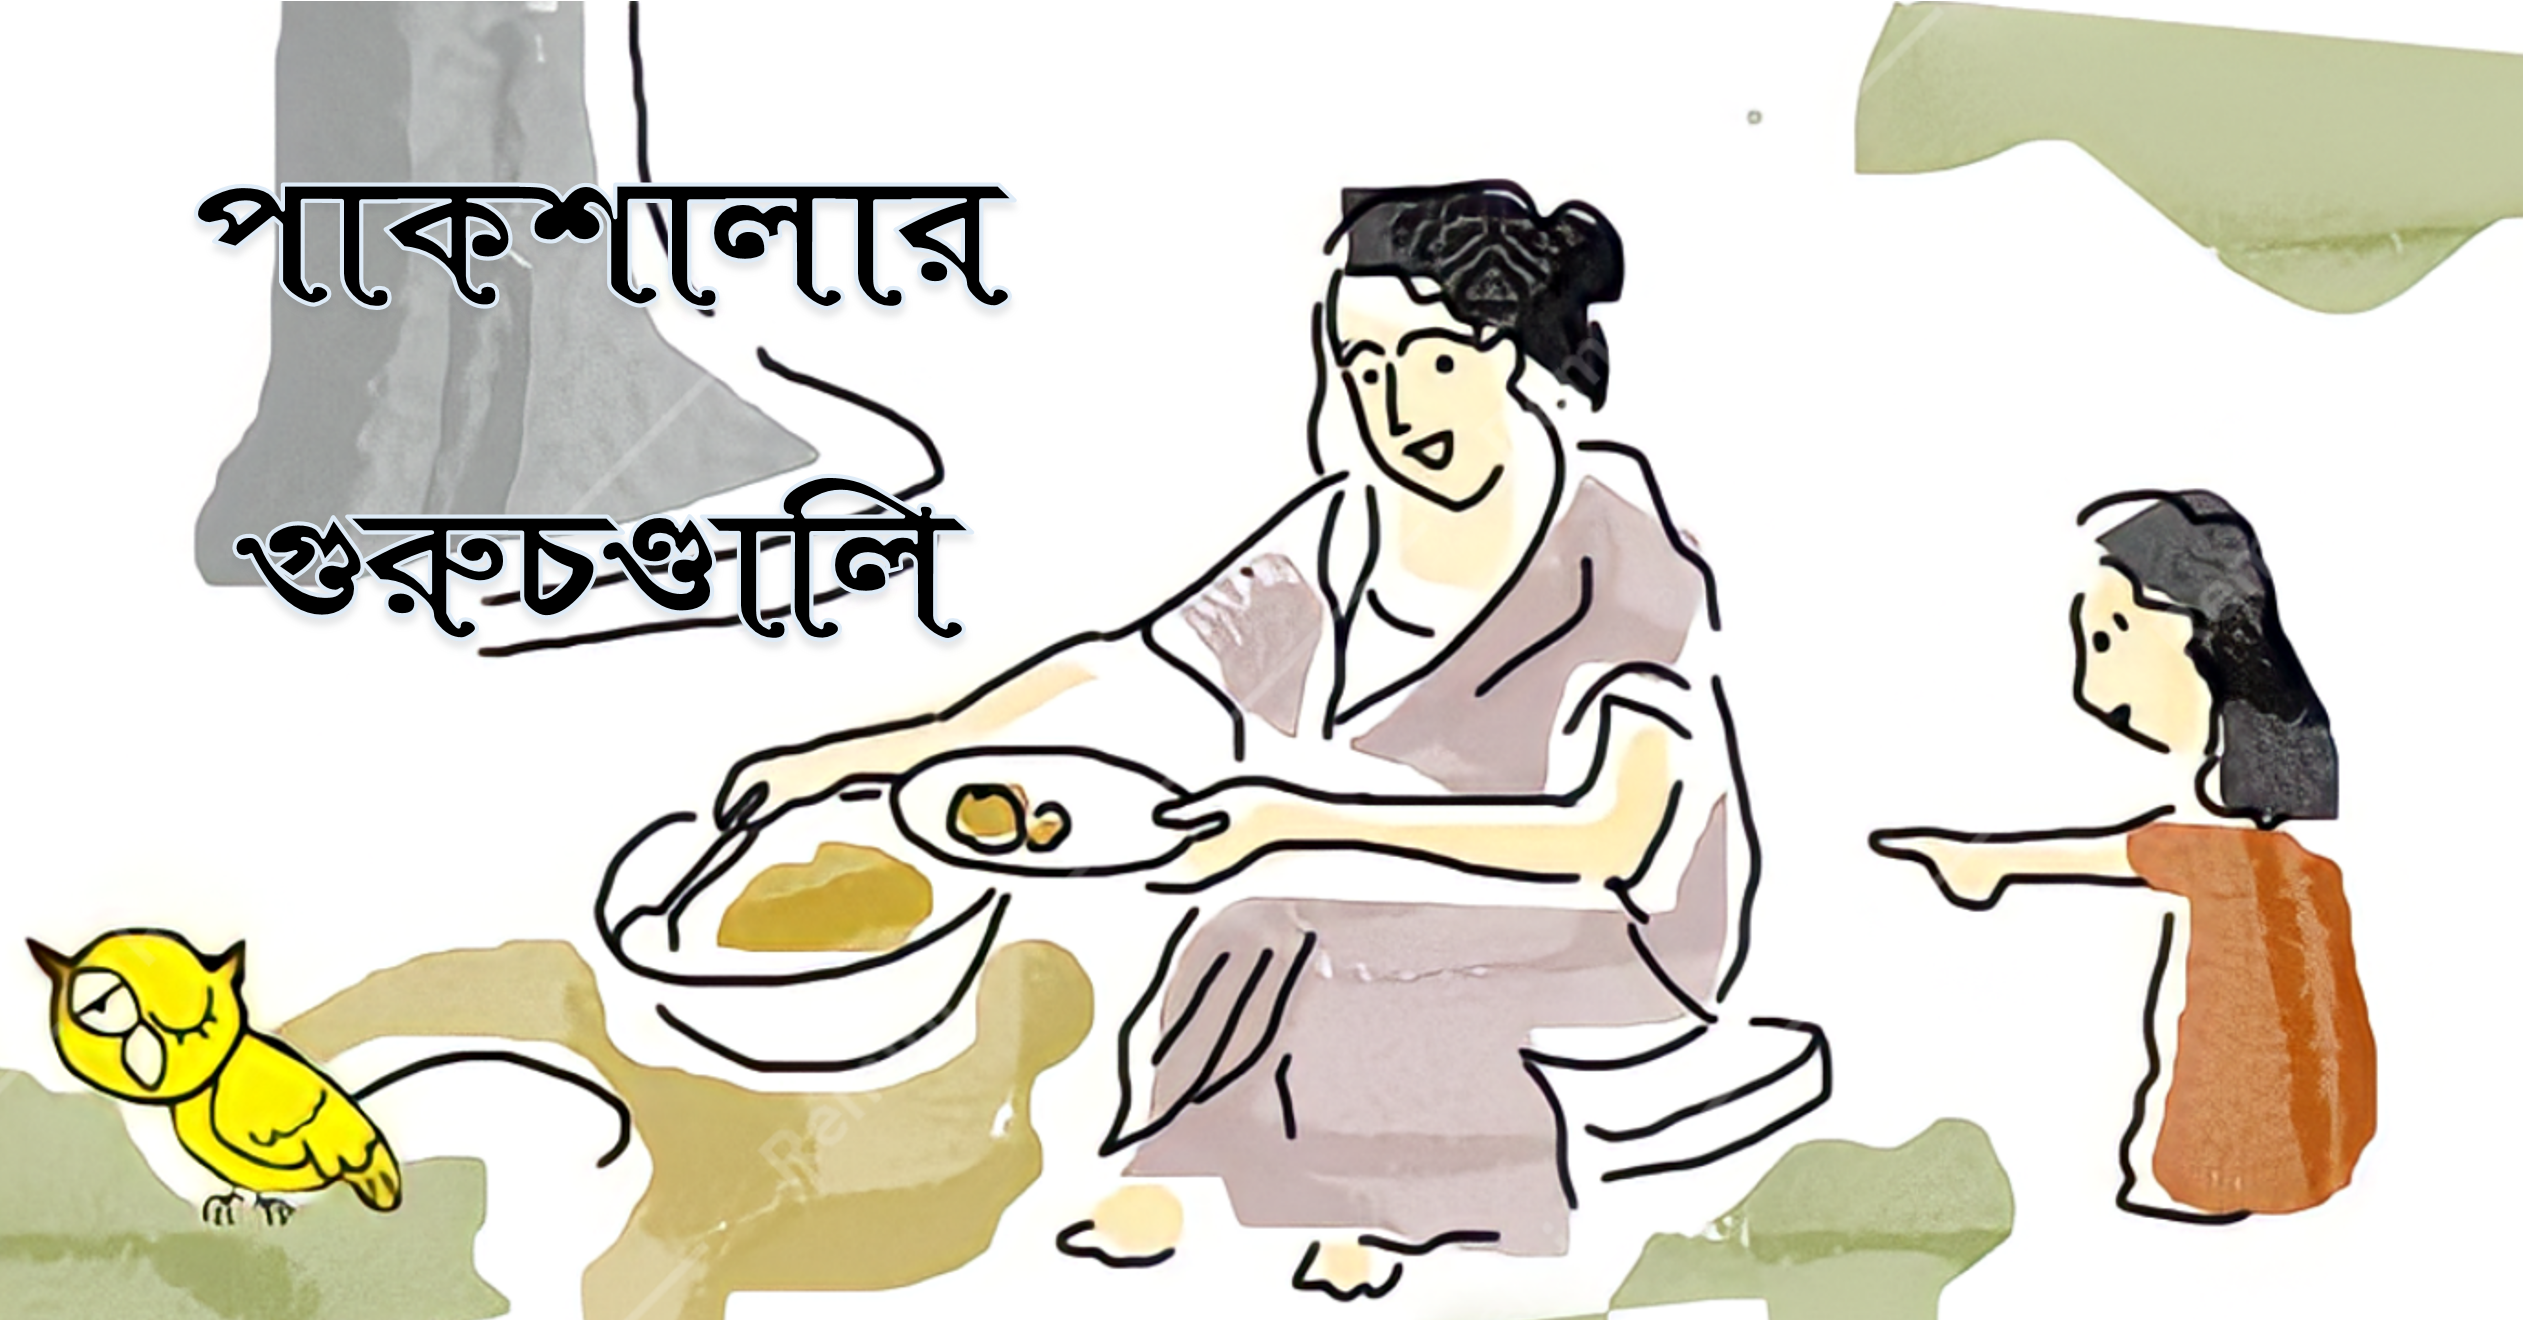
\includegraphics[width=\linewidth]{Images/DemoPic1.png}
	\caption{\small \textbf{ডেমো ক্যাপশন}}
\end{figure}

জীবের মধ্যে সবচেয়ে সম্পূর্ণতা মানুষের। কিন্তু সবচেয়ে অসম্পূর্ণ হয়ে সে জন্মগ্রহণ করে। বাঘ ভালুক তার জীবনযাত্রার পনেরো- আনা মূলধন নিয়ে আসে প্রকৃতির মালখানা থেকে। জীবরঙ্গভূমিতে মানুষ এসে দেখা দেয় দুই শূন্য হাতে মুঠো বেঁধে।

মানুষ আসবার পূর্বেই জীবসৃষ্টিযজ্ঞে প্রকৃতির ভূরিব্যয়ের পালা শেষ হয়ে এসেছে। বিপুল মাংস, কঠিন বর্ম, প্রকাণ্ড লেজ নিয়ে জলে স্থলে পৃথুল দেহের যে অমিতাচার প্রবল হয়ে উঠেছিল তাতে ধরিত্রীকে দিলে ক্লান্ত করে। প্রমাণ হল আতিশয্যের পরাভব অনিবার্য। পরীক্ষায় এটাও স্থির হয়ে গেল যে, প্রশ্রয়ের পরিমাণ যত বেশি হয় দুর্বলতার বোঝাও তত দুর্বহ হয়ে ওঠে। নূতন পর্বে প্রকৃতি যথাসম্ভব মানুষের বরাদ্দ কম করে দিয়ে নিজে রইল নেপথ্যে।

মানুষকে দেখতে হল খুব ছোটো, কিন্তু সেটা একটা কৌশল মাত্র। এবারকার জীবযাত্রার পালায় বিপুলতাকে করা হল বহুলতায় পরিণত। মহাকায় জন্তু ছিল প্রকাণ্ড একলা, মানুষ হল দূরপ্রসারিত অনেক। 
\begin{quotation}
	\textit{জীবের মধ্যে সবচেয়ে সম্পূর্ণতা মানুষের। কিন্তু সবচেয়ে অসম্পূর্ণ হয়ে সে জন্মগ্রহণ করে। বাঘ ভালুক তার জীবনযাত্রার পনেরো- আনা মূলধন নিয়ে আসে প্রকৃতির মালখানা থেকে। জীবরঙ্গভূমিতে মানুষ এসে দেখা দেয় দুই শূন্য হাতে মুঠো বেঁধে।\\
	মানুষ আসবার পূর্বেই জীবসৃষ্টিযজ্ঞে প্রকৃতির ভূরিব্যয়ের পালা শেষ হয়ে এসেছে। বিপুল মাংস, কঠিন বর্ম, প্রকাণ্ড লেজ নিয়ে জলে স্থলে পৃথুল দেহের যে অমিতাচার প্রবল হয়ে উঠেছিল তাতে ধরিত্রীকে দিলে ক্লান্ত করে। প্রমাণ হল আতিশয্যের পরাভব অনিবার্য। পরীক্ষায় এটাও স্থির হয়ে গেল যে, প্রশ্রয়ের পরিমাণ যত বেশি হয় দুর্বলতার বোঝাও তত দুর্বহ হয়ে ওঠে। নূতন পর্বে প্রকৃতি যথাসম্ভব মানুষের বরাদ্দ কম করে দিয়ে নিজে রইল নেপথ্যে।\\
	মানুষকে দেখতে হল খুব ছোটো, কিন্তু সেটা একটা কৌশল মাত্র। এবারকার জীবযাত্রার পালায় বিপুলতাকে করা হল বহুলতায় পরিণত। মহাকায় জন্তু ছিল প্রকাণ্ড একলা, মানুষ হল দূরপ্রসারিত অনেক।}
\end{quotation}
জীবের মধ্যে সবচেয়ে সম্পূর্ণতা মানুষের। কিন্তু সবচেয়ে অসম্পূর্ণ হয়ে সে জন্মগ্রহণ করে। বাঘ ভালুক তার জীবনযাত্রার পনেরো- আনা মূলধন নিয়ে আসে প্রকৃতির মালখানা থেকে। জীবরঙ্গভূমিতে মানুষ এসে দেখা দেয় দুই শূন্য হাতে মুঠো বেঁধে।

মানুষ আসবার পূর্বেই জীবসৃষ্টিযজ্ঞে প্রকৃতির ভূরিব্যয়ের পালা শেষ হয়ে এসেছে। বিপুল মাংস, কঠিন বর্ম, প্রকাণ্ড লেজ নিয়ে জলে স্থলে পৃথুল দেহের যে অমিতাচার প্রবল হয়ে উঠেছিল তাতে ধরিত্রীকে দিলে ক্লান্ত করে। প্রমাণ হল আতিশয্যের পরাভব অনিবার্য। পরীক্ষায় এটাও স্থির হয়ে গেল যে, প্রশ্রয়ের পরিমাণ যত বেশি হয় দুর্বলতার বোঝাও তত দুর্বহ হয়ে ওঠে। নূতন পর্বে প্রকৃতি যথাসম্ভব মানুষের বরাদ্দ কম করে দিয়ে নিজে রইল নেপথ্যে।

মানুষকে দেখতে হল খুব ছোটো, কিন্তু সেটা একটা কৌশল মাত্র। এবারকার জীবযাত্রার পালায় বিপুলতাকে করা হল বহুলতায় পরিণত। মহাকায় জন্তু ছিল প্রকাণ্ড একলা, মানুষ হল দূরপ্রসারিত অনেক।

\vskip 30pt
\scriptsize
	\textbf{সূত্র:}
	\begin{enumerate}%[label={}]
		\item ১২০৫-১২০৬ খ্রিস্টাব্দের দিকে ইখতিয়ার উদ্দিন মুহম্মদ বখতিয়ার খলজী নামের একজন তুর্কী বংশোদ্ভূত সেনাপতি রাজা লক্ষ্মণ সেনকে পরাজিত করে সেন রাজবংশের পতন ঘটান।
		\item ১৭৫৭ খ্রিস্টাব্দে ব্রিটিশ ইস্ট ইন্ডিয়া কোম্পানি পলাশীর যুদ্ধে জয়লাভের মাধ্যমে বাংলার শাসনক্ষমতা দখল করে
		\item ১৮৫৭ খ্রিস্টাব্দের সিপাহী বিপ্লবের পর কোম্পানির হাত থেকে বাংলার শাসনভার ব্রিটিশ সাম্রাজ্যের সরাসরি নিয়ন্ত্রণে আসে
		\item ভারতীয় উপমহাদেশের দেশভাগের সময় ১৯৪৭ খ্রিস্টাব্দে ধর্ম গরিষ্ঠতার ভিত্তিতে পুনর্বার বাংলা প্রদেশটিকে ভাগ করা হয়। পাকিস্তান এর প্রদেশ হিসাবে জন্ম নেয় পূর্ব পাকিস্তান 
		\item ১৯৭১ সালে ৯ মাস ব্যাপী রক্তক্ষয়ী যুদ্ধের মাধ্যমে পাকিস্তানী হানাদার বাহিনীকে পরাজিত করে স্বাধীনতা লাভ করে বাংলাদেশ 
	\end{enumerate}



	\normalsize
\phantomsection
\chapter{দ্বিতীয় অধ্যায়ের নাম}
%\addcontentsline{toc}{chapter}{দ্বিতীয় অধ্যায় (সূচীপত্রে)}
\markright{হেডার দ্বিতীয়}

\section{প্রথম পরিচ্ছেদ}

\BanglaDummyText
\begin{table}[ht]
	\centering
	\begin{tabular}{|c|c|c|}
		\hline
		&	হরিপুর (ছাত্র সংখ্যা)	&	আদর্শ (ছাত্র সংখ্যা) \\
		\hline
		ছেলে	&	৮৪  (৮০ জন) 		&	৮৫ (২০ জন) \\
		\hline
		মেয়ে	&	৮০  (২০ জন) 		&	৮১  (৮০ জন)\\
		\hline
	\end{tabular}
\end{table}

\BanglaDummyText

\section{দ্বিতীয় পরিচ্ছেদ}

\BanglaDummyText

\begin{figure}
	\centering
	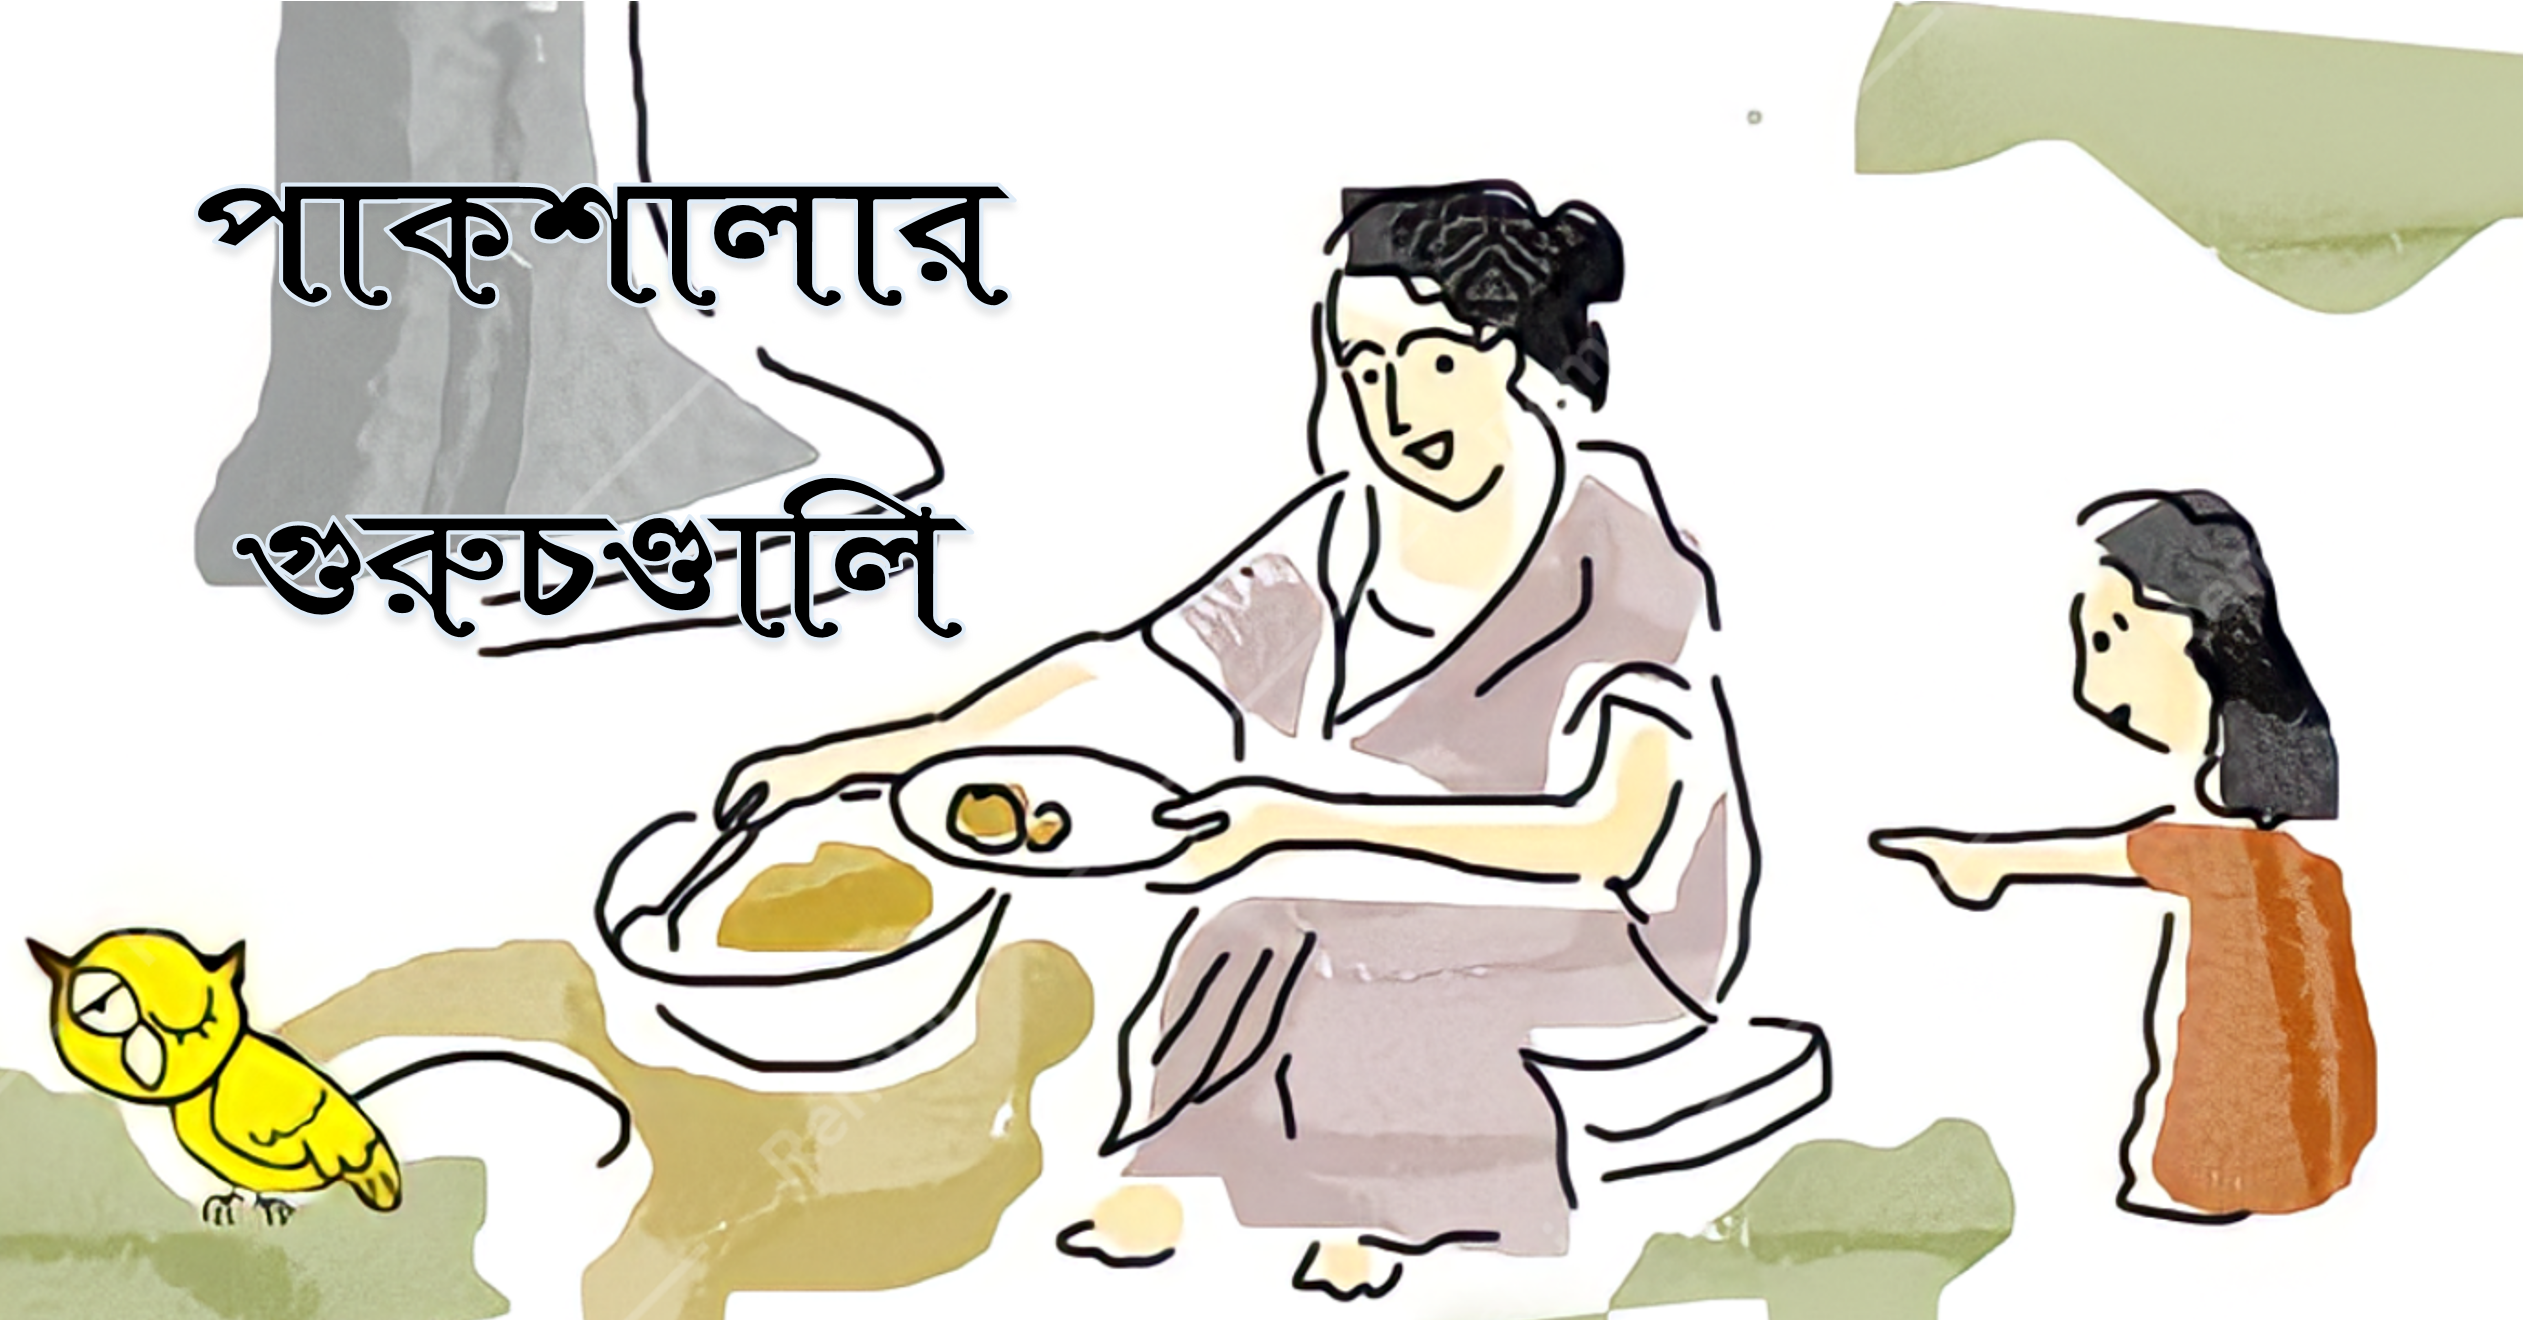
\includegraphics[width=\linewidth]{Images/DemoPic1.png}
	\caption{\small \textbf{ডেমো ক্যাপশন}}
\end{figure}

\BanglaDummyText
\begin{quotation}
	\textit{\BanglaDummyText}
\end{quotation}
\BanglaDummyText

\vskip 30pt
\scriptsize
\textbf{সূত্র:}
\begin{enumerate}%[label={}]
	\item ১২০৫-১২০৬ খ্রিস্টাব্দের দিকে ইখতিয়ার উদ্দিন মুহম্মদ বখতিয়ার খলজী নামের একজন তুর্কী বংশোদ্ভূত সেনাপতি রাজা লক্ষ্মণ সেনকে পরাজিত করে সেন রাজবংশের পতন ঘটান।
	\item ১৭৫৭ খ্রিস্টাব্দে ব্রিটিশ ইস্ট ইন্ডিয়া কোম্পানি পলাশীর যুদ্ধে জয়লাভের মাধ্যমে বাংলার শাসনক্ষমতা দখল করে
	\item ১৮৫৭ খ্রিস্টাব্দের সিপাহী বিপ্লবের পর কোম্পানির হাত থেকে বাংলার শাসনভার ব্রিটিশ সাম্রাজ্যের সরাসরি নিয়ন্ত্রণে আসে
	\item ভারতীয় উপমহাদেশের দেশভাগের সময় ১৯৪৭ খ্রিস্টাব্দে ধর্ম গরিষ্ঠতার ভিত্তিতে পুনর্বার বাংলা প্রদেশটিকে ভাগ করা হয়। পাকিস্তান এর প্রদেশ হিসাবে জন্ম নেয় পূর্ব পাকিস্তান 
	\item ১৯৭১ সালে ৯ মাস ব্যাপী রক্তক্ষয়ী যুদ্ধের মাধ্যমে পাকিস্তানী হানাদার বাহিনীকে পরাজিত করে স্বাধীনতা লাভ করে বাংলাদেশ 
\end{enumerate}

\backmatter
	\clearpage
\pagenumbering{gobble}
\markboth{}{}

\makeatletter
\newlength\drop
\newcommand*{\titleGM}{\begingroup% Gentle Madness
	\drop = 0.08\textheight
	\vspace*{0.5\baselineskip}
	%\vfill
	\hbox{%
		\hspace*{0.2\textwidth}%
		\rule{1pt}{0.4\textheight}
		\hspace*{0.05\textwidth}%
		\parbox[b]{0.75\textwidth}{
			\vbox{%
				\vspace{\drop}
				{\hspace{-25pt}\raggedright\normalsize\@title\par
				}
				\vskip\baselineskip
				\centering
				{\@author%\par
				}
				\vskip16\baselineskip
				{\raggedright\@date\par}
				\vspace{0.04\textheight}
			}% end of vbox
		}% end of parbox
	}% end of hbox
	%\vfill
	\null
	\endgroup}
\makeatother


\title{ বইটির আংশিক আর্থিক দায়িত্ব নিয়ে দত্তক নিয়েছেন:}
\author{\large\textbf{\guruAdoptionList}}
\date{\scriptsize \textit{মানুষের বই পড়ার অভ্যাস নাকি হারিয়ে যাচ্ছে। অথচ বইয়ের দাম বেড়ে চলেছে লাফিয়ে লাফিয়ে। বোঝা যায়, ক্ষুদ্র একটা পাঠকবৃত্তকে সম্বল করে চলছে বই-ব্যাবসা। ছোট্টো পাঠকবৃত্ত, তাই বইয়ের দাম বেশি, আবার বইয়ের দাম বেশি বলে পাঠকসংখ্যা কম, তৈরি হচ্ছে এরকম এক অন্তহীন দুষ্টচক্র।\\
		এই চক্রব্যূহ থেকে বেরিয়ে আসার জন্যই আমাদের দাওয়াই ‘দত্তক’। গুরুচণ্ডা৯ লেখক-পাঠক সমবায়ে বিশ্বাসী, মুনাফায় নয়। গুরুচণ্ডা৯র শুভানুধ্যায়ীরা নিয়মিতভাবেই এক বা একাধিক বইয়ের সম্পূর্ণ বা আংশিক দায়ভার বহন করেন, যার পোশাকি নাম ‘দত্তক’। বাজারচলতি বইয়ের চেয়ে কমে আসে আমাদের বইয়ের দাম। পৌঁছে যায় আরও বহু মানুষের কাছে।\\
		আপনি কি এই মিথোজীবিতার সক্রিয় অংশীদার হতে চান? গুরুচণ্ডা৯-র বই দত্তক নিতে চান?\\
		যোগাযোগ করুন: guruchandali@gmail.com\\
		হোয়াটসঅ্যাপ: +৯১ ৯৩৩০৩ ০৮০৪৩}}
	
		\titleGM
%	\newpage \ % Use this to add blank pages at the end of the document.

\end{document}
